\section{Behavior Model}
\label{sec:behavior}


Our behavior model in a dynamic scene consists of three parts. 
One is the behavior of single object, which is represented by the statistics of the object motion (rotations/translations) interpreted from its orientations and positions in frames.
%
The second is the behavior of a group of object, which means the correlations of the statistics of the motions of objects. Their supporting/proximity relationship or arrangements of a group of objects keep consistent. 
%
c. The relationship variations caused by motion of the objects in the set of point clouds. In other words, the behavior of the object relationship. For example, the support relationship of vase can change from one desktop to another desktop or so.  

\comment{
\subsection{Static Object Relations}

The static object relations are defined in two-level. The first level is the pairwise relation between any two objects, supporting and proximity. The second is the structural group which describes the spatial distribution of a subset consisting of more than two objects, such as symmetric or uniformly distributed objects.

\subsubsection{Pairwise Object Relations}
}
\subsection{Pairwise Object Relations}
\label{sec:pairwise_relation}


In a cluttered indoor scene, there are many pairs of objects that usually co-occur in the scene with some typical geometric relations in a long time period. 
%
In our system, we consider two types of pairwise relations, which are commonly used to describe object relations in many previous methods~\cite{Fisherscenesynth12,Silberman:ECCV12,Xu13sig,xu_sig14}.


\paragraph{Support} $SR(\objmodel_a,\objmodel_b)$ indicates that $\objmodel_a$ is supported by $\objmodel_b$. We use a Gaussian function to indicate the distribution of $\objmodel_a$ on the supporting surface of $\objmodel_b$;
%
In each frame, we check any pair of objects connected by a surface. 
Typically, smaller object is supported by the larger one, the upper object is supported by the bottom object.
%
%We scale the supported $\objmodel_b$ into a unit square with factor $s_x,s_y$, then scale
We transform the object been supported $\objmodel_a$ into the local coordinates of its support object $\objmodel_b$ to get its location $\mathbf{x}_a$ and orientation $\theta_a$.
%
According to all the examples of this pair in the input frames, we compute a Gaussian function
\begin{equation}
	\label{eq:sr_ab}
	SR(\objmodel_a,\objmodel_b) = \mathcal{N}_{position}(\mathbf{\mu}_{x},\Sigma_{x}) \mathcal{N}_{orientation}(\mu_{o},\sigma_{o})
\end{equation} 
Each relation has a confidence or frequency $w$ in all the frames. 




\paragraph{Proximity} $PR(\objmodel_a,\objmodel_b)$ indicates $\objmodel_a$ is close to $\objmodel_b$ in with a Gaussian function $\mathcal{N}(\mu,\sigma)$ including position $x,y$ in the local coordinate system of $\objmodel_a$ and the orientation $\theta_b$ of $\objmodel$  in the local coordinate system of $\objmodel_b$, defined as 
%\xj{only considering object pairs that are close enough, say $dis(o_a,o_b)<Thr_{proximity}$?} 
%
\begin{equation}
	\label{eq:proximity_ab}
	PR(\objmodel_a,\objmodel_b) = \mathcal{N}_{position}(\mathbf{\mu}_{x},\Sigma_{x}) \mathcal{N}_{orientation}(\mu_{o},\sigma_{o}).
\end{equation} 



If the background floor and wall are taken into account for pairwise relations, the relation between a single object and the background is actually the behavior of this object itself.




\subsection{Group Behavior}
\label{sec:groupbehavior}

Based on all the extracted pairwise relation, a directed graph $G(V,E)$ is constructed to encode the mutual relations of all the objects in the scene, as shown in Figure~\ref{fig:geometric_graph}. 
Each node is an object model in the scene.   
%
Each directed edge represents a pairwise geometric relation between two objects. 
%
The information carried in each edge includes:
\begin{enumerate}
	\item \textbf{Relation type}:  supporting or proximity. Each edge is directed from a small object to an larger object indicating that the small object is usually associated with a larger object. 
	%
	\item \textbf{Edge weight}: is the frequency of that two objects co-occur in the scene. We define it 
	\begin{equation}
		w(i\to j)= \frac{c(i\to j)}{K}	\end{equation}
	where $c(i\to j)$ is the total counts of that two objects co-occur and follow the relation defined by the edge in all the frames. $K$ is the number of all frames.
	\comment{Note: if there is only one frame where a cup is placed on a cabinet while it is always placed on an office desk, there will be a supporting edge from the cup to the cabinet but with very low weight. Do we remove this weak edge using threshold? This truncation can be done in the reliable group selection as well.}
	
	\item \textbf{Relation description}: Associated with each edge, the statistics of the spatial relations defined in Sec.~\ref{sec:pairwise_relation} is also stored. 
\end{enumerate}



%\subsubsection{Structural Group}
%\label{sec:group-relation}

A \textbf{structural group} $G_s$ is defined as a \emph{complete graph} in which every pair of nodes in connected by a unique edge, to describe the mutual relations between nodes in a subset.
%\xj{The completeness of a structural group guaranttees the compactness of each subgroup. } 
%
From the directed graph $G(V,E)$, a set of structural groups can be extracted. There are many potential structural groups in $G$. The smallest structural group is an edge connecting two nodes. 
%with a reliability $\rho_{sg}$. 
%
However, we only focus on reliable structural groups for further application, such as layout re-arrangement, unusual event detection, etc. 
%
The reliability of a structural group $G_s(V_s,E_s)$ with $k$ objects is defined as defined as
\begin{equation}
	\label{eq:reliability_sg}
	\rho_{sg} = \big(\prod_{e_i \in E_s} {w(e_i)}\big)^{\frac{1}{k}}
\end{equation}



\begin{figure}
	\centering
	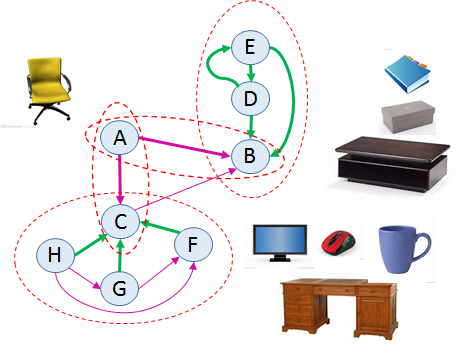
\includegraphics[width=0.98\columnwidth]{figures/geometric_graph.png}
	\caption{Construction a directed geometric graph from pairwise relations. Green edges indicate supporting relations. Purple edges represent proximity relations. The edge width indicates the frequency of each relation. Each dashed ellipse represents a structural group. \redemph{The pair (B,C) should be very weak because they are far away from other other, and can be removed. Otherwise, (A,B,C) is another structural group.}}
	\label{fig:geometric_graph}
\end{figure}


\comment{
\paragraph{Multiple instances}
%

\xj{More explaination of multiple instances.}
%
When there are multiple instances of the same object model co-occur in an indoor scene, for example, two chairs with a table, as shown in Figure~\ref{fig:multiple_instance_sg}, the two instances are registered to the same object model in the segmentation and registration step. 
%
In the construction of the geometric graph, each node is an object model. So the two chairs are represented as the one node B, as shown in Figure~\ref{fig:multiple_instance_sg}(b). The pairwise relation between the table and the chair is proximity, with the spatial relation can be modeled by \redemph{two Gaussians}. 

However, this representation implicitly discards the behavior relations between the objects of the same type. 
Moreover, the geometric graph could not exactly reflect the layout of the target scene.            
\xj{If two instances are treated as two distince nodes, how to recover the correspondences between frames?}    

We introduce the another type of structural group $G_{mi}$, as shown in Figure~\ref{fig:multiple_instance_sg}(c).
A structural group with multiple instances have the following properties:
\begin{enumerate}
	\item The structural group have more than one object instances which are registered to the same geometry model. 
	\item The multiple instances having the same geometric relation with the same host object. For example, two chairs must always close to the same desk in the scene, or two boxes are supported by the same table.
\end{enumerate}

\xj{Not all instances follow this definition. Only the instances following these properties compose a structural group, as Figure~\ref{fig:multiple_instance_a} shows.}


For a structural group with multiple instances, the geometric relation of each instance with its supporting object is computed as following:
\begin{enumerate}
	\item For an object model, find all the frames where multiple instances co-occur. 
	\item Find the same host object to all of the instances. 
	\item In the local coordinate system of the host object, map the positions and orientations of all the instances. 
	\item If $k$ instances co-occur in the scene, then recover a GMM model with $K$ Gaussians for the $k$ instances.  
\end{enumerate}

\begin{figure}
	\centering
	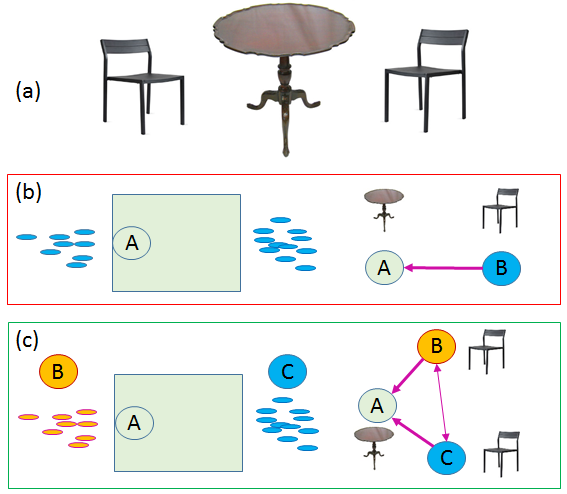
\includegraphics[width=\columnwidth]{figures/instance_graph_2.png}
	\caption{A structural group with multiple instances co-occur in the scene.}
	\label{fig:multiple_instance_sg}
\end{figure}


\begin{figure}
	\centering
	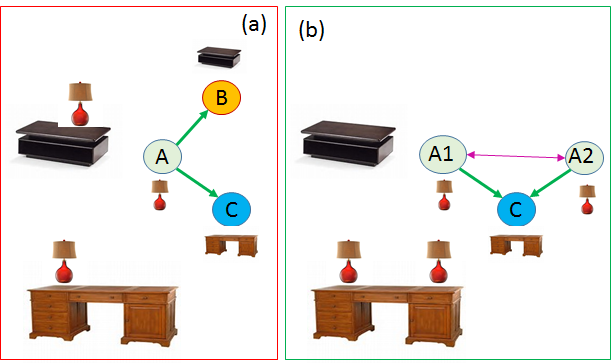
\includegraphics[width=\columnwidth]{figures/instance_graph_3.png}
	\caption{Not all instances should be described using structural graph with multiple instances. (a) The two lamps can be represented using one node (A), which are separately supported by two other objects (B and C). (b) If the two instances are highly correlated, it is much better to clearly represent their spatial relations using two distinct nodes (A1, A2). }
	\label{fig:multiple_instance_a}
\end{figure}

}


\comment{
	\begin{algorithm}
		\caption{Behavior analysis given object registration}
		\label{alg:behavior}
		\begin{algorithmic}[1]
			\State {Input: A set of RGBD patches $\patch_{i,k}$, $k=1,\ldots,K$ frames.}
			\State {Input: A set of object models $\objmodel_{i}$, $i=1,\ldots,M$.}
			\State {Input: correspondence between each patch and object models $\patch_i = \mathbf{T}_i\objmodel_j$.} 
			\State {Compute the \emph{supporting relations} between any pair of object models $SR(\objmodel_i,\objmodel_j)$;}
			\State {Compute the \emph{proximty relations} between any pair of patches $PX(\objmodel_i,\objmodel_j)$;}
			\State {Build a directed graph $G(V,E)$ consisting of all the objects in the scene.}
			\State {Extract structural group from $G(V,E)$ with high reliability: $\rho_{sg} > T_{sg}$.}
			\State {Extract structural group with multiple instances. }
			
		\end{algorithmic}
	\end{algorithm}
}







